\section{问题二：场馆与开球时段协同优化}

\subsection{三维指派与候选域}

设比赛、场馆和参考时段集合为 $\mathcal I,\mathcal V,\mathcal S$。仅当场馆安保能力满足比赛需求时保留候选
\begin{equation}
\Omega=\{(i,v,s):L_v^{sec}\ge L_i^{req}\},
\end{equation}
并建立 $x_{ivs}\in\{0,1\}$；$y_v$ 表示场馆是否启用。当前数据形成 $85680$ 个三维布尔变量。场馆和时段同时决定当地日期、票务、转播、旅行与风险，因此不把问题拆成两个相互独立的贪心步骤。

比赛 $i$ 在场馆 $v$ 的预计上座为 $N_{iv}=\min(N_i^{pre},K_v)$。票务、转播和成本原值为
\begin{align}
T^0(x)&=\sum_{(i,v,s)\in\Omega}x_{ivs}P_{r(i)}^0N_{iv},\\
B^0(x)&=\sum_{(i,v,s)\in\Omega}x_{ivs}V_i^{pre}u_{r(i)}g_s^{prime}w_{r(i)}^{sponsor},\\
C^0(x,y)&=\sum_v10^6c_v^{setup}y_v+
\sum_{(i,v,s)\in\Omega}x_{ivs}\left(10^6c_v^{op}+10^5L_i^{req}c_v^{sec}\right).
\end{align}
费用统一换算为美元，场馆启用费只计一次。附件中所有场馆的最小承办数均为 $2$，故每个可行方案必启用全部 $16$ 个场馆，启用费在本数据中是共同常数。

\subsection{旅行、风险与公平指标}

旅行严格使用题面特殊口径。距离、旅行时间和时区差先在全部合法球队--轮次--候选场馆组合上分别 Min--Max，再按 $0.5,0.3,0.2$ 合成。第一轮从球队代表地出发；第二、三轮对球队 $t$ 和本轮场馆 $v$，以前一轮全部安保合格场馆为起点：
\begin{equation}
\bar q_{trv}=\frac{1}{|\mathcal V_{t,r-1}^{qual}|}
\sum_{u\in\mathcal V_{t,r-1}^{qual}}q_{uv},\qquad
q\in\{distance,time,timezone\}.
\end{equation}
每场取双方平均并对 $72$ 场求均值得到 $D$，不能替换成上一轮实际所选场馆的路径。

单场执行风险为
\begin{equation}
r_{iv}=0.5c_v^{climate}+0.3\frac{N_{iv}}{K_v}+0.2\frac{L_i^{req}}{L_v^{sec}},
\end{equation}
整套赛程取均值 $R$。悬念 $U$ 为 $72$ 场竞技悬念指数均值，吸引力 $H$ 为吸引力指数除以 $100$ 后的均值。若球队 $t$ 的黄金时段和大容量场馆次数分别为 $n_t^{prime},n_t^{large}$，公平惩罚为
\begin{equation}
F=\frac12\frac{\max_t n_t^{prime}-\min_t n_t^{prime}}3+
\frac12\frac{\max_t n_t^{large}-\min_t n_t^{large}}3.
\end{equation}
黄金时段取 $80$ 个候选时段中得分最高的 $20$ 个，大容量场馆取 $16$ 个场馆中容量最高的 $4$ 个；阈值并列未跨越名额切点。

\subsection{确定性的全部候选组合 Min--Max}

旧实现用六个限时辅助排程的对偶最好界作 $T,B,C$ 端点，等价表达式会改变搜索路径和端点，因而不适合作为可复现的评价尺度。本文改为直接枚举全部合法三元候选。对 $k\in\{T,B,C\}$，逐场在 $\Omega_i$ 中取候选最小和最大后汇总：
\begin{equation}
k_{min}=\sum_{i\in\mathcal I}\min_{(v,s)\in\Omega_i}k_i(v,s),\qquad
k_{max}=\sum_{i\in\mathcal I}\max_{(v,s)\in\Omega_i}k_i(v,s),
\end{equation}
其中 $C$ 的两端同时加入全部必启用场馆的一次性成本。任何满足联合约束的赛程都是该候选笛卡尔域的子集，故其指标必落在包络内；该计算不调用求解器、没有时间限制和随机性。得到
\begin{align}
T^0&\in[281888385,285910470],\\
B^0&\in[150900200.787,367190488.581],\\
C^0&\in[47730000,63910000].
\end{align}
三项用 $(k-k_{min})/(k_{max}-k_{min})$ 归一化；若端点相等则按题意置零。$U,H,D,F,R$ 已按上述定义位于 $[0,1]$。最终目标为
\begin{equation}
\max Z_2=0.25T+0.25B+0.15U+0.10H-0.08C-0.07D-0.06F-0.04R.
\end{equation}

\subsection{硬约束与求解设置}

模型逐项施加：每场恰好一次指派；同一场馆同一 UTC 时刻至多一场；球队按三轮顺序参赛且相邻轮至少休息 $60$ 小时；场馆当地日负荷和总负荷满足附件上下限；不建立安保不合格候选；同一时段比赛数不超过转播容量；第三轮高安保比赛逐参考日不超过动态容量；任意球队黄金时段次数极差不超过 $2$。核心形式包括
\begin{align}
\sum_{v,s}x_{ivs}&=1,&
\sum_i x_{ivs}&\le1,\\
\tau_{t,r+1}-\tau_{tr}&\ge60,&
\max_t n_t^{prime}-\min_t n_t^{prime}&\le2.
\end{align}
场馆日容量按所选 UTC 时刻转换到场馆 IANA 时区后的当地日期计算，动态资源容量则按附件参考日计算，两类日期不混用。

所有浮点目标系数乘 $10^6$ 转为整数。CP-SAT 固定单线程和随机种子 $20260813$，最长运行 $1800$ 秒，相对间隙阈值 $0.5\%$；先在宽轮次窗口内求可行提示，再在完整 $80$ 时段域求主目标。Python 3.11 的两次独立进程分别用时约 $173$ 与 $177$ 秒，Python 3.12 的干净环境复现用时约 $580$ 秒；三次均达到相同停止准则并生成逐字节相同的正式 CSV。

\subsection{结果与可执行性}

主方案原值为 $T^0=285581790$、$B^0=323423207.006$、$C^0=53075000$ 美元；八项标准化指标为
\begin{equation}
\begin{aligned}
(T,B,U,H)&=(0.918281,0.797646,0.461436,0.639699),\\
(C,D,F,R)&=(0.330346,0.201797,0.333333,0.416678).
\end{aligned}
\end{equation}
从而 $Z_2=0.484946$，高于同约束可行基线 $0.350742$。缩放目标的可行值为 $17811471$、最好界为 $17883841$，相对证书间隙约 $0.406\%$；因此 `OPTIMAL` 只按预设 $0.5\%$ 停止口径解释，不声称零间隙精确最优。

\begin{figure}[htbp]
\centering
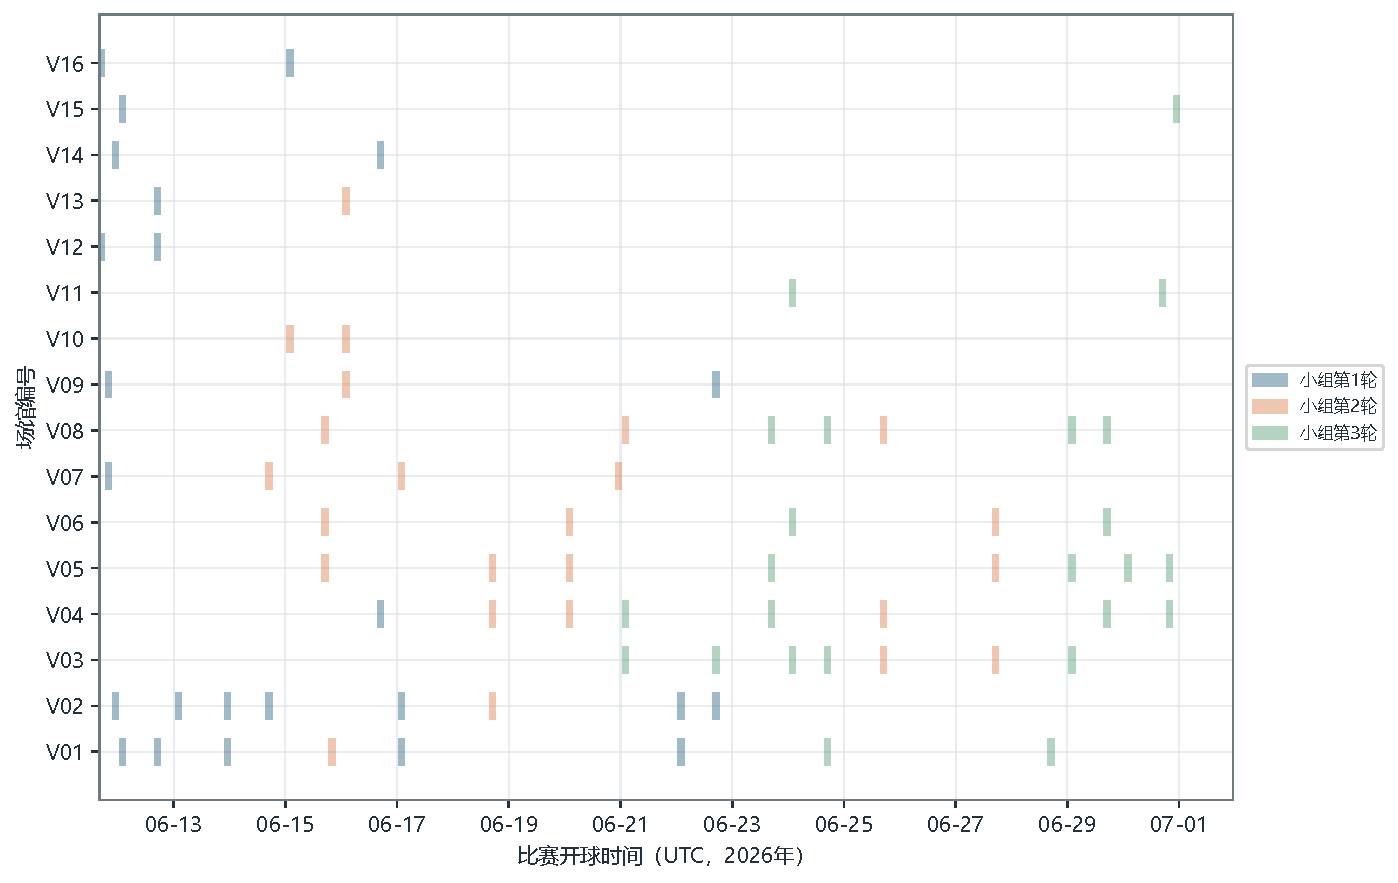
\includegraphics[width=0.88\textwidth,height=0.66\textheight,keepaspectratio]{../figures/fig_q2_schedule_gantt.pdf}
\caption{问题二最终 72 场 UTC 排程}
\label{fig:q2-schedule-gantt}
\end{figure}

\begin{table}[H]
\centering
\caption{问题二关键约束复算与裕度}
\label{tab:q2-constraint-audit}
\small
\begin{tabular}{lrrrrc}
\toprule
约束族 & 实际值 & 界值 & 单位 & 最小裕度 & 状态 \\
\midrule
最小轮间休息 & 63.000 & 60.000 & 小时 & 5.0\% & 通过 \\
场馆承办下界 & 0.000 & 0.000 & 剩余场 & 0.0\% & 通过 \\
场馆承办上界 & 0.000 & 0.000 & 剩余场 & 0.0\% & 通过 \\
场馆单日本地容量 & 1.000 & 1.000 & 最大利用率 & 0.0\% & 通过 \\
场馆安保等级 & 0.000 & 0.000 & 等级余量 & 0.0\% & 通过 \\
时段转播容量 & 0.000 & 0.000 & 剩余场 & 0.0\% & 通过 \\
第三轮高安保日容量 & 0.000 & 0.000 & 比例余量 & 0.0\% & 通过 \\
黄金时段公平极差 & 1.000 & 2.000 & 场 & 50.0\% & 通过 \\
\bottomrule
\end{tabular}
\vspace{2pt}
\noindent\begin{minipage}{0.96\textwidth}\footnotesize 注：裕度为按各约束自身上限归一化后的最小剩余比例；零表示约束在最紧样本上取等。\end{minipage}
\end{table}


独立从正式 CSV 复算：$72$ 个比赛编号完整且唯一，场馆--UTC 冲突为 $0$，最小轮间休息为 $63$ 小时；$16$ 个场馆各承办 $2$--$8$ 场，场馆当地日、安保、时段转播和第三轮高安保容量均无违反。黄金时段次数极差为 $1$，大容量场馆次数极差为 $1$。逐场票务、转播、旅行和风险字段与附件公式的最大数值误差低于 $10^{-8}$，总目标只写在 CSV 第一条记录。
